\documentclass[a4paper]{article}

\usepackage[francais,english]{babel}
\usepackage[T1]{fontenc}
\usepackage[]{fullpage}
\usepackage{graphicx}
\usepackage{hyperref}
\usepackage[utf8]{inputenc}
\usepackage{subfigure}

\makeatletter
\def\thickhrulefill{\leavevmode \leaders \hrule height 1pt\hfill \kern \z@}
\def\maketitle{%
  \null
  \thispagestyle{empty}%
  \vskip 1cm
  \begin{flushright}
        \normalfont\Large\@author
  \end{flushright}
  \vfil
  \hrule height 2pt
  \par
  \begin{center}
        \huge \strut \@title \par
  \end{center}
  \hrule height 2pt
  \par
  \vfil
  \vfil
  \null
\begin{center}
\Huge{Placement constraints for a better QoS in clouds}
\end{center}
\begin{figure}[!ht]
	\centering
	
\includegraphics[scale=.45]{imgs/cloud.png}
\end{figure}
\vfil
\begin{figure}[!ht]
	\centering
	
\includegraphics[scale=.5]{imgs/polytech.png}
\end{figure}
\vfil
\begin{description}
	\item[Entreprise] Université de Nice-Sophia Antipolis
	\item[Lieu] Sophia-Antipolis, France
	\item[Responsable] Fabien Hermenier, équipe OASIS,
		\href{mailto:fabien.hermenier@unice.fr}{fabien.hermenier@unice.fr}
\end{description}
\cleardoublepage
}
\makeatother
\author{Mathieu Bivert, CSSR, \href{mailto:bivert@essi.fr}{bivert@essi.fr}}
\title{PFE: Cahier des charges (DOW)}

\begin{document}
\maketitle

\selectlanguage{francais}
\begin{abstract}
Dans le cadre de la répartition de machines virtuelles sur un ensemble de
serveurs physiques, ce projet vise à formaliser puis implémenter des
contraintes de placement, portant sur le type de systèmes de virtualisation.
\end{abstract}

\selectlanguage{english}
\begin{abstract}
Within the framework of placing virtual machines on a set of physical servers,
this project aims to formalize and to implement placement constraints,
relative to the type of different virtualization systems.
\end{abstract}

\tableofcontents
\newpage
\section{Description du projet}
\subsection{Contexte de travail}
Le monde industriel étant de plus en plus informatisé, la qualité des
réseaux s'améliorant, les sociétés informatiques tendent à  louer des
structures informatiques accessibles à distance.

Les hébergeurs de services informatiques étant spécialisées dans la
maintenance de ces structures, elles sont plus performantes qu'une société
spécialisée dans la construction d'automobiles par exemple.
Cette dernière a alors tout interêt a déporter la charge de la conception
et de la maintenance de ses systèmes d'informations à une entreprise
de services. Cette dernière pourra offrir à ses clients des solutions
personnalisées, et peu coûteuses par rapport à une gestion \og manuelle \fg.

% Une conséquence sur le matériel utilisé est le remplacement de
% dizaines de postes de bureau par des clients légers, peu cher et
% gourmand en ressources. En effet, ceux-ci sont uniquement chargés
% de fournir à l'utilisateur un affichage, un clavier, une souris et
% une connexion réseau, le calcul pouvant être effectué sur des serveurs
% distants.

À noter que cependant que toutes les entreprises n'ont pas forcément
interêt à exporter leur centre de traitement de l'information : par
exemple des structures reposant sur des données hautement confidentielles
(recherche de pointe, armée, état, etc.).

Le terme de \og cloud \fg\ correspond à un certain nombre de serveurs
physiques et de logiciels, utilisés par une entreprise de services. Ces
dernières se déclinent en plusieurs types selon le(s) service(s) qu'elles
proposent:
\begin{description}
	\item[SaaS] Software As A Service, fournir un logiciel
		(eg. un client email : Gmail\footnote{\url{https://gmail.com}});
	\item[PaaS] Platform As A Service, fournir un ensemble de logiciels et services
		(eg. accès aux Google Apps\footnote{\url{https://www.google.com/enterprise/apps/business/}});
	\item[IaaS] Infrastructure As A Service, fournir des ressources matérielles
		(eg. Amazon EC2\footnote{\url{https://aws.amazon.com/ec2/}});
	\item[DaaS] Data As A Service, fournir un accès à des données
		(eg. Dropbox\footnote{\url{https://www.dropbox.com/}});
	\item[] $\ldots$
\end{description}

En particulier, un cloud \textit{IAAS} fournit à l'utilisateur l'accès
à un ensemble de systèmes d'exploitations. Ces derniers sont très
souvent virtualisés, ce qui présente l'avantage de pouvoir faire tourner
plusieurs OS sur un même serveur physique. La virtualisation repose sur
un \textit{hyperviseur}, c'est-à-dire un moniteur de machines virtuelles (VM), dont
le but est réaliser l'isolation entre les différentes VMs et de les administrer.
L'administration consiste à démarrer, arrêter, migrer, régler les ressources des
VMs.

Par exemple, la figure \ref{hubertfxen} montre l'hyperviseur \textit{Xen}~\cite{barham2003xen}
sous NetBSD en train de virtualiser un FreeBSD, deux NetBSDs et une Debian.
\begin{figure}[!ht]
	\centering
	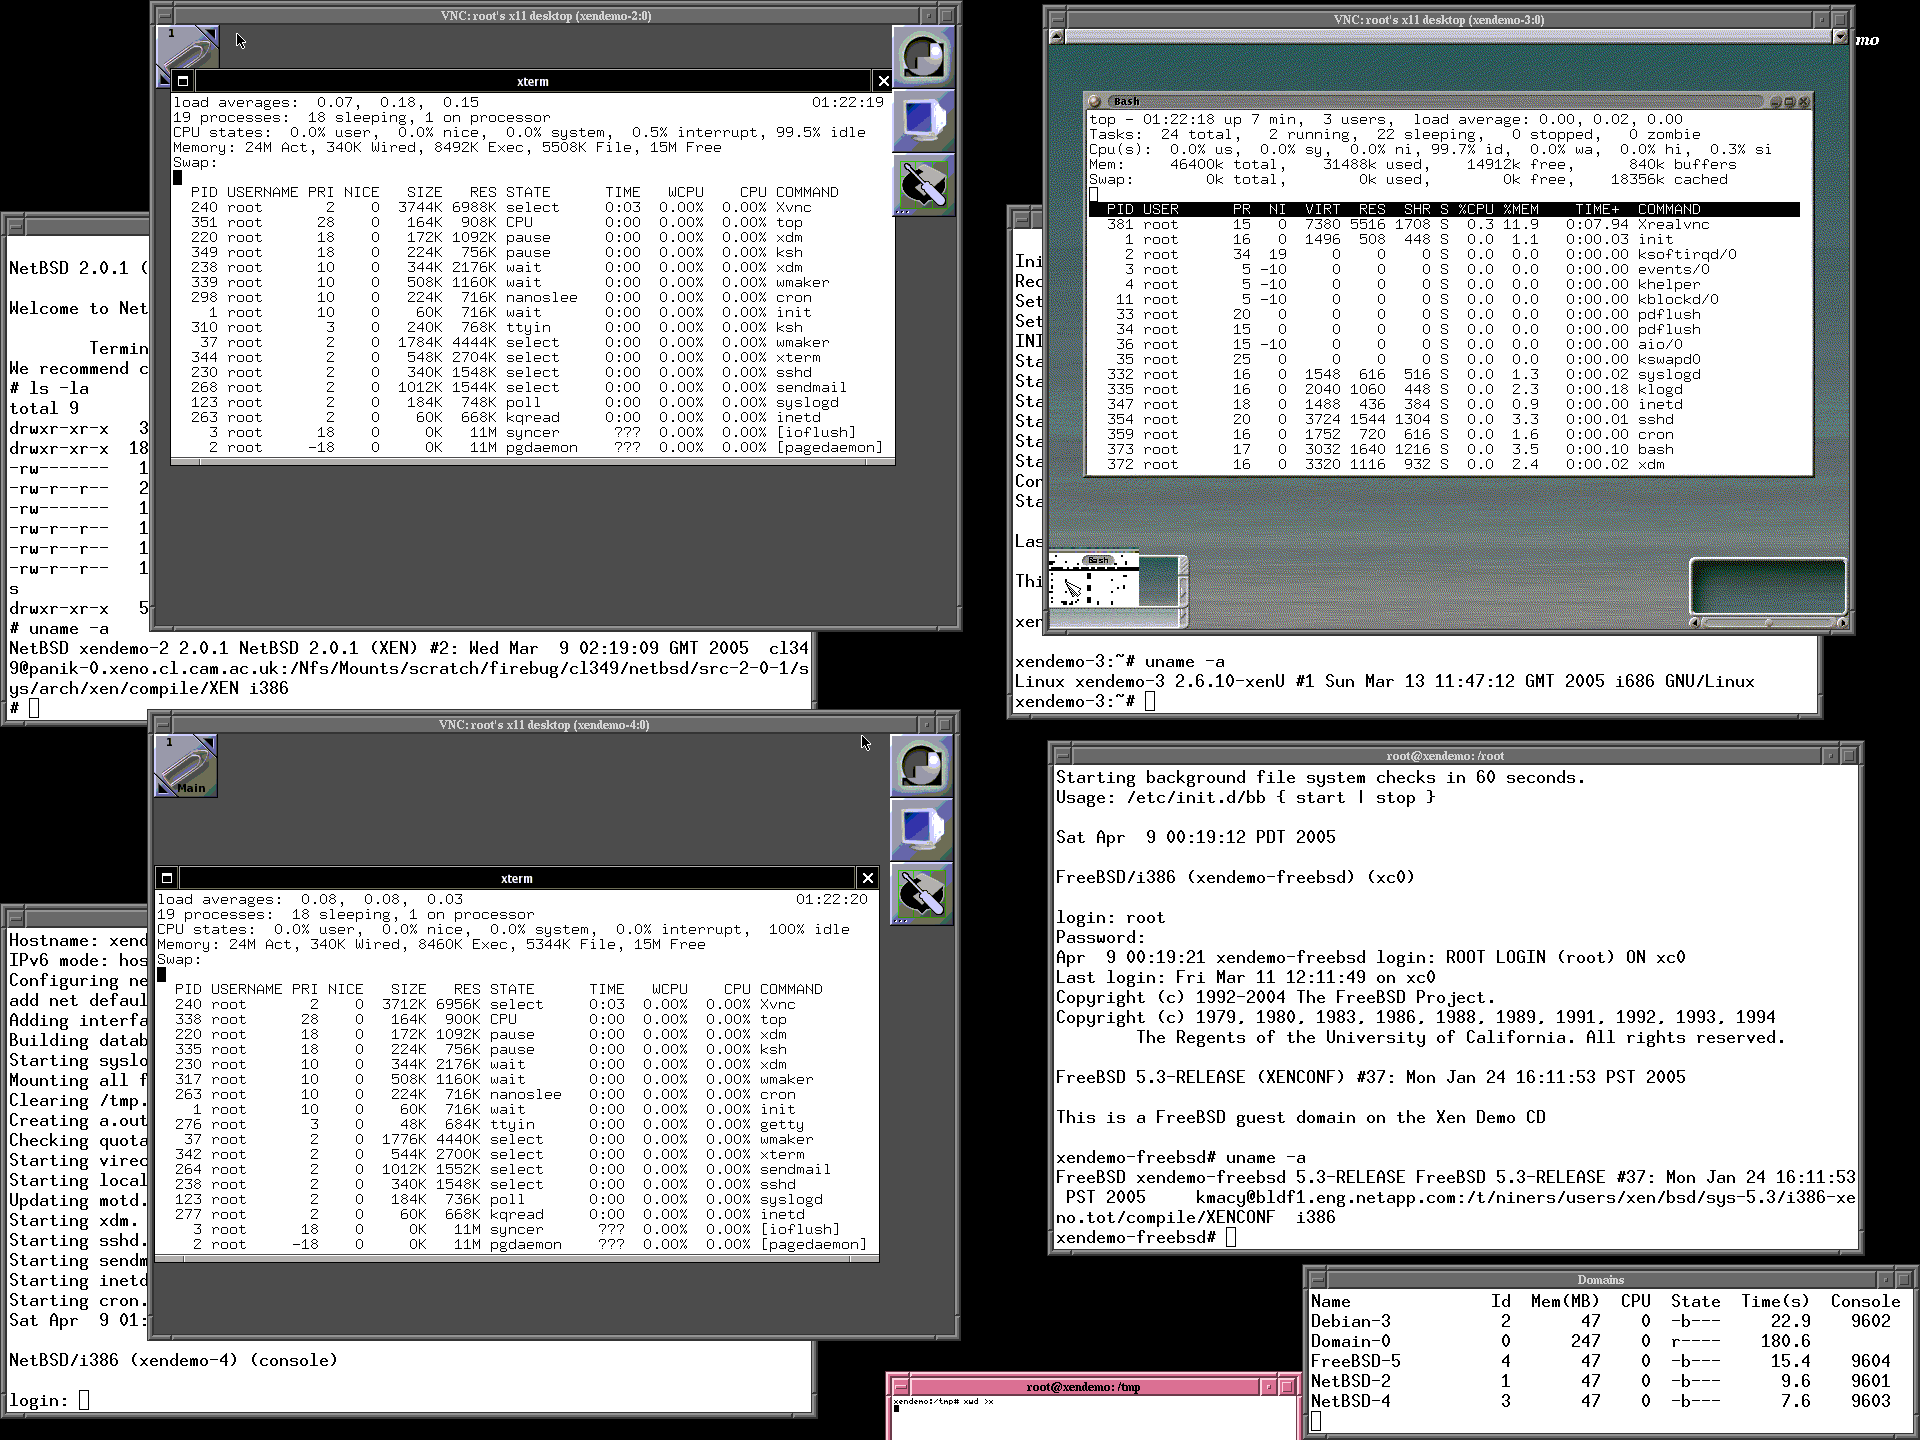
\includegraphics[scale=.17]{imgs/hubertf-xen.png}
	\caption{\label{hubertfxen} Virtualisation avec Xen; trois clients
		VNC \protect\footnotemark sont lancés pour accéder aux VMs}
\end{figure}

Une problématique pour les gestionnaires d'IAAS est donc de pouvoir placer
correctement un ensemble donné de VMs sur un ensemble de serveurs physiques.
Ce placement n'est pas libre : il est régit par un ensemble de contraintes
qui doivent être satisfaites.

\subsection{Motivations}
La virtualisation présente plusieurs avantages:
\begin{itemize}
	\item sur une application dite $n$-tiers, il est possible
	de placer chaque tiers sur une VM, et éventuellement d'en faire
	des duplications, ce qui améliore la robustesse de l'application.
	Par exemple, n cas de défaillance d'un serveur physique, il est
	stratégique d'avoir placé le réplicat d'un serveur de base de
	données sur un serveur différent de l'original;
	\item l'admninistration et la gestion des machines est simplifiée :
	il y a moins de hardware, donc moins de maintenance physique;
	la possibilité de pouvoir cloner/charger/décharger à la volée des
	VMs permet d'améliorer la QoS facilement. Notamment, dans le cas
	où l'administrateur doit effectuer une opération de maintenance sur
	un serveur physique, il va devoir migrer~\cite{clark2005live} les VMs
	sur un autre serveur;
	\item chaque application peut être répartie sur une VM différente.
	Ainsi, si une application est compromise, elle a moins de chances
	de pouvoir compromettre d'autres applications que si elles étaient
	toutes lancées sous un même OS;
	\item utilisation plus performante du matériel, lorsqu'un ordinateur
	puissant peu être utilisé au maximum de ses performances en faisant
	tourner plusieurs systèmes d'exploitations. Cependant, utiliser un
	serveur à $99\%$ de ses capacités n'est pas judicieux, puisque celui-ci
	sera alors incapable d'assurer une augmentation de charge. Il est donc
	impératif d'éviter une saturation;
	\item $\ldots$
\end{itemize}

% for hubertfxen; can't be in \caption; may need te be moved later to
% appears on the same page than the graphics
\footnotetext{\url{http://www.hep.phy.cam.ac.uk/vncdocs/index.html}}

La question de la répartition des machines virtuelles sur les machines
physiques se pose alors pour des raisons diverses et variées:
\begin{description}
	\item[maintenance] un serveur physique peut tomber en panne, ou
		nécessiter une réparation, auquel cas les programmes
		tournant dessus doivent être migré ailleurs, afin de
		garantir au client une certaine qualité de service (QoS);
	\item[sécurité] il peut s'avérer risquer pour un programme d'un
		client traitant des données sensibles (eg. données bancaires)
		de se retrouver au même endroit qu'un programme d'un
		autre client;
	\item[évolution des besoins] où au cours d'un certain intervalle de
		temps, les besoins en puissance de calcul d'une entreprise
		peuvent augmenter (suite à une plus grande popularité par
		exemple), ou encore, augmentation brusque et irrégulière
		de la charge à des heures de pointes;
	\item[économie d'énergie] où il peut être avantageux de réduire
		le nombre de serveurs physiques allumés, pour maximiser
		le rendement des autres machines physiques du cloud;
	\item[QoS] où, à l'inverse de l'économie d'énergie, il est bon
		de garder des ressources supplémentaires disponibles immédiatement,
		de façon à ne pas perdre de temps (et donc en QoS) à redémarrer
		un autre serveur;		
	\item[licence] les entreprises fournissant les systèmes de virtualisation
		proposent des licences selon différents critères (eg. nombre de
		machines virtuelles lancées, utilisation de ressources (CPU, RAM, etc.));
	\item[plateforme] plusieurs plateformes de virtualisations sont disponibles
		(eg. Xen, VMWare, Citrix); une autre contrainte sur la
		répartition des machines virtuelles se pose alors, un serveur
		physique ne faisant tourner qu'un seul type de plateforme;
	\item[] $\ldots$
\end{description}

Enfin, on notera que ces besoins fluctuent au cours du temps; les systèmes
de placement doivent donc être flexibles, au moins à deux niveaux.
D'abords, ils doivent être \textit{configurable} afin de prendre en compte
les spécificités et les propriétés, éventuellement variables des applications
et du datacenter. Une deuxième propriété d'\textit{extensibilité} est nécessaire,
ce afin d'être capable de supporter de nouvelles fonctionnalités au fur et à mesure
de l'évolution des besoins.

\subsection{Défis}
Afin de compléter le manque de fonctionalités, l'ajout de contraintes à
la volée est requise. Malgré un contexte fortement combinatoire (eg.
le placement d'une VM influençant le placement d'autres VMs, la viabilité
des contraintes), l'approche se doit d'être suffisamment flexible.

La solution proposée par l'algorithme BtrPlace~\footnote{\url{http://btrp.inria.fr/sandbox/about.html};
il est mis en place dans Entropy~\cite{herm2009}, un manager de clusters}
va dans ce sens : il utilise la programmation
par contrainte pour trouver une solution viable au placement, en un temps
assez \og court \fg\ pour gérer un datacenter conséquent ($5000$ serveurs, $30000$
VMs en $3$ minutes) de nouvelles contraintes peuvent être ajoutées sous
formes de plugins Java en une trentaine de lignes de code, etc.

\subsection{Objectifs}
Actuellement, les trois/quatres derniers points cités ne sont pas forcément
formalisés/implémentés complètement. Le projet consiste donc à choisir l'un
de ces domaines et à l'ammener vers une forme satisfaisante.

Le dernier point est celui sur lequel se porte ce projet. Le travail sera
d'autant plus original que les questions d'économies d'énérgies sont actuellement
très prisées par les chercheurs au détriment des autres.

Au sein d'une infrastructure, plusieurs types d'hyperviseurs/de VMs doivent
être supportés. Afin de satisfaire le critère de flexibilité, on peut avoir
besoin de changer le système de supervision des VMs d'un serveurs dynamiquement.
Par exemple, on peut désirer vouloir garantir une certaines proportions
d'une plateforme donnée, un nombre maximum de plateformes d'un certain type, etc.

Dans l'état actuel, BtrPlace est incomplet : il ne permet pas de gérer le type
des VMs/plateformes ni les étapes de reconfiguration. Dans ce sujet,  on
se propose donc dans un premier temps, d'étendre le modèle actuel
pour supporter le typage des infrastructures. C'est-à-dire, fournir
une implémentation de base permettant d'associer un type à une machine
virtuelle, et un ensemble de types possibles pour un serveur. En effet,
ces derniers peuvent ne pas supporter n'importe quel hyperviseur.

Dans un second temps, on modélise et implémente un ensemble de contraintes
pour contrôler les plateformes selon leur type. Par exemple, on peut limiter le
nombre de plateformes d'un type donné, interdire un changement de type
sur un serveur, etc.

\subsection{Scénarios}
On reprend l'exemple précèdent sur la figure \ref{reconf} avec des
informations plus proches de ce qu'il se passe en réalité.
\begin{figure}[!ht]
	\centering
	\subfigure[Avant la reconfiguration] {
		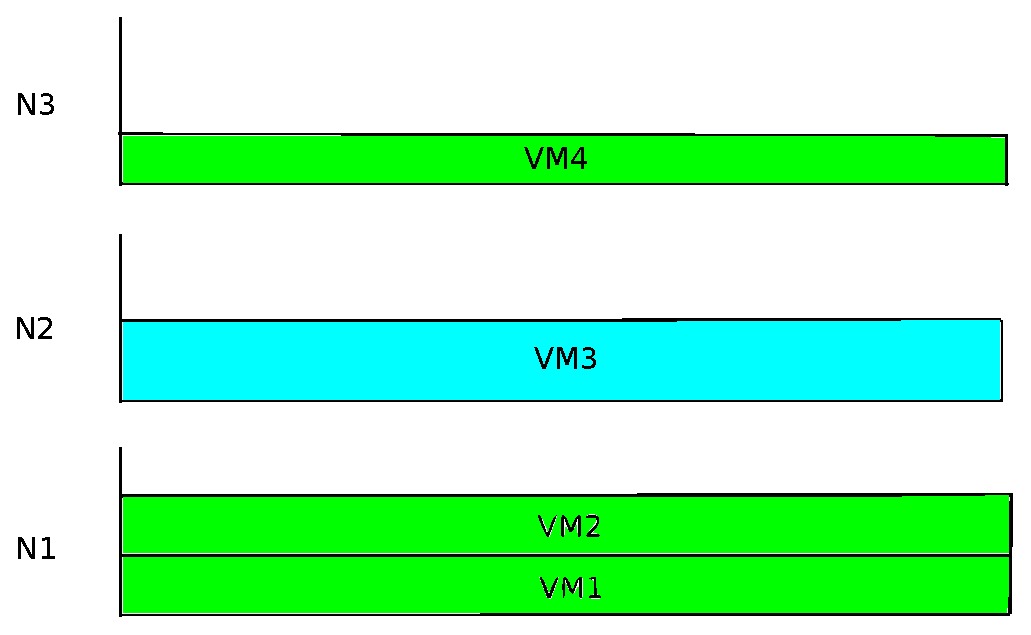
\includegraphics[scale=.40]{imgs/startreconf.eps}
		\label{startreconf}
	}
	\subfigure[Après la reconfiguration] {
		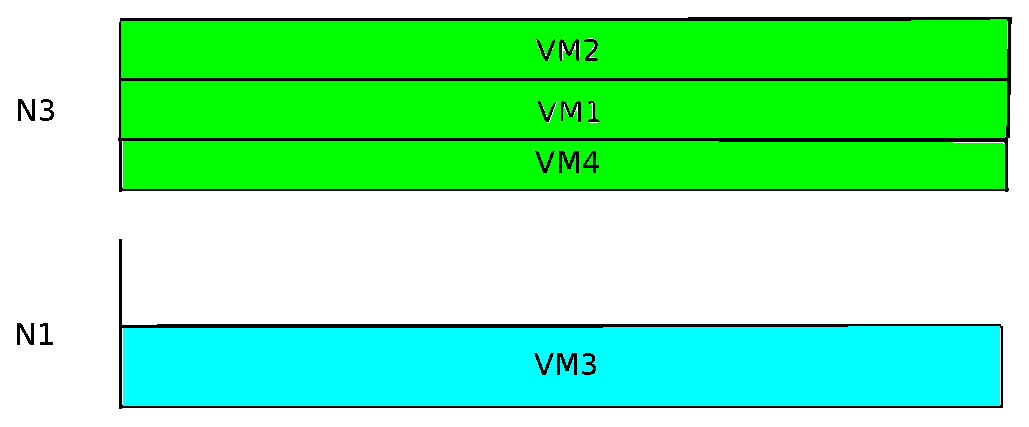
\includegraphics[scale=.40]{imgs/endreconf.eps}
		\label{endreconf}
	}
	\caption{\label{reconf} Exemple de changement de système de
		virtualisation. En vert des VMs Xen, en cyan une VM VMWare}
\end{figure}

Sur le diagramme \ref{startreconf}, on souhait mettre le serveur physique
$N_2$ hors-ligne pour des questions de maintenance. On utilise pour cela
la contrainte \textit{offline($N_i$);}\footnote{\url{http://www-sop.inria.fr/members/Fabien.Hermenier/btrpcc/offline.html}}.

Comme aucun serveur VMWare n'est disponible, il est nécessaire de supprimer
un serveur Xen, capable d'accueillir $VM_3$, par exemple $N_1$. Les machines
virtuelles situées sur ce dernier, $VM_1$ et $VM_2$,  doivent dans un premier
temps être migrées sur un autre serveur.

Puis, $N_1$ doit s'éteindre et redémarrer en changeant son système
de virtualisation. Enfin, la $VM_3$ est déplacée sur $N_1$, et $N_2$ peut
être éteint, pour arriver dans l'état décrit par le diagramme \ref{endreconf}.

\subsection{Critère de succès}
L'extension apportée à BtrPlace devra supporter correctement les problèmes
de dépendances en le placement des VMs, le typage des serveurs et l'éventuel
changement dynamique de type de ceux-ci. Enfin, les contraintes doivent être
censées, bien définies et répondre à des besoins concrets.

\section{État de l'art}
(XXX pas lus, pas de citations)
\subsection{Description générale}
Historiquement, les gestionnaires de placement se sont concentrés sur
le placement des VMs selon leurs besoins en ressources (CPU, RAM, BP, etc.),
tout en cherchant à réduire la consommation énergétique

Traditinonellement, ces approches reposent sur des algorithmes ad'hoc rapides
pour répartir les VMs. D'autres algorithmes plus flexible ont vu le jours
suite au demande des clients, par exemple portant sur la fiabilité des
applications.

Jung et al. proposent d'utiliser une fonction d'utilité pour les
applications à haute disponibilité et performance. Leur solution
porte sur la défaillance de serveurs physique, mais pas sur des
changements de charge. Un algorithme glouton calcule le nombre de
réplicats nécessaires pour chaque composant de l'application, de
façon à satisfaire les besoins en temps de latence du réseau et
en performance. Les réplicats peuvent être placés sur des racks
ou des datacenters différents selon le degré voulu de fiabilité.
(phrase pas claire). Ajouter de nouveaux paramètres, tels que la
gestion des types de serveurs, demande de revoir l'algorithme
de reconfiguration. Les tests sont limités à un datacenter d'une
douzaine de serveurs.

VMWare DRS donne à l'adminstrateur un accès à $4$ contraintes
similaire à \textit{ban}, \textit{fence}, \textit{gather} et
\textit{spread}. Cependant, leur version de \textit{spread}
ne garantit pas que lors du déplacement d'une VM, l'ancienne
version ne va pas tourner en même temps que la nouvelle.
DRS n'est pas prévu pour être étendu, et $5$ des contraintes
de BtrPlace y sont manquantes. De plus, DRS ne choisit pas
automatiquement en fonction des propriétés d'une VM entre
une re-instantiation ou une migration à chaud. (induced re-location?)
Enfin, DRS ne permet d'administrer que des clusters de $32$
serveurs.

Entropy est à l'origine de BtrPlace. La programmation par contraintes
est utilisée pour placer les VMs sur un nombre minimum de serveur.
L'ordonnancement des actions nécessaires à la migration étant calculé
avec une heuristique ad'hoc, il est impossible d'ajouter des
contraintes telles que \textit{spread}, qui affectent l'ordonnancement.
Finalement, toutes les VMs en marche sont prises en compte lors
de la résolution d'un mauvais placement, ce qui limite le nombre
de serveurs gérés à quelques centaines.

Récemment, de nouvelles approches plus flexibles ont vu le jour;
elles permettent d'intégrer des contraintes de placement à la
demande. Bin et al. utilise aussi la programmation par contraintes
pour fournir un gestionnaire de placement modulaire. Ils
permettent une haute-disponibilité en guarantissant qu'à chaque instant,
un certains nombre de serveurs sera disponible pour satisfaire
la consommation de ressources des VMs et les contraintes de
déplacement. Lorsqu'un serveur a de fortes chances de tomber en panne,
les VMs sont migrés sur un autre capable de les satisfaire. Le modèle
proposé ne supporte pas les contraintes portant sur la gestion de
l'état des serveurs, l'ordonnancement des actions ou encore sur la
façon dont les VMs sont migrées. Enfin, l'extensibilité n'a été
vérifiée que pour $32$ serveurs physiques et $128$ VMs au maximum.

Quelques aspects théoriques de BtrPlace ont été étudié au préalable,
avec un premier prototype prenant en compte les ressources allouées
aux VMs, leur placement et l'étape de migration. \cite{herm2012}
étends ce travail en montrant que BtrPlace est capable de gérer
des datacenters de plusieurs centaines de serveurs. BtrPlace
est donc à l'heure actuelle le gestionnaire le plus efficace en
ce qui concerne le placement de VMs, tout en rendant possible
de contrôler l'état des serveurs et les sur-allocations de ressources.
L'addition d'une dizaine de nouvelles contraintes répondant à
ces besoins démontre une extensibilité correcte. L'utilisation
d'une heuristique basée sur une optimisation de filtre (XXX quésaco?)
rends BtrPlace jusqu'à $20$ fois plus rapide sur la gestion de
datacenters composés de $2500$ serveurs.

\section{Méthodologie et planification}
\subsection{Stratégie générale}
\subsection{Découpage en lots}
bis repetita: trouver un bon formalisme; définir et implémenter
\subsection{Plannification}
gantt
\subsection{Livrables associés au projet}
\begin{table}
\centering
\begin{tabular}{c|c|c|c|c}
	Id & Titre du livrable & Lot(s) & Nature & Date \\
	\hline
	\hline
	$D_0$ & Cahier des charges & $1$ & Document & $S_4$ \\
	\hline
	$D_1$ & Gestion du typage et du déploiement & $1$ & Document & $?$ \\
	\hline
	$D_2$ & Ensemble de contraintes & $1$ & Document et Logiciel & $?$ \\
	\hline
	$D_3$ & Rapport de management & $1$ & Document & $S_{20}$ \\
	\hline
	$D_4$ & Diaporama de présentation finale & $1$ & Document & $S_{20}$ \\
\end{tabular}
\end{table}

\subsection{Jalons}
\begin{table}
\centering
\begin{tabular}{c|c|c|c|c}
	Id & Jalon de fin de phase & Lot(s) & Date & Vérification \\
	\hline
	\hline
	$J_0$ & planification & $1$ & $S_4$ & $D_0$ \\
	\hline
	$J_1$ & formalisation & $1$ & $S_n$ & $D_1$ partiel \\
	\hline
	$J_2$ & implémentation & $1$ & $S_{n+k}$ & $D_2$, $D_1$ partiel \\
	\hline
	$J_3$ & projet & $1$ & $S_{20}$ & $D_1$, $D_2$, $D_3$ et $D_4$ \\
\end{tabular}
\end{table}

\section{Description de la mise en œuvre du projet}
\subsection{Interdépendance des lots et tâches}
bis repetita: trouver un bon formalisme; définir et implémenter
\subsection{Description des lots}
bis repetita: trouver un bon formalisme; définir et implémenter
\subsection{Résumé de l'effort}
\subsection{Gestion du risque}

\section{Participants}
\subsection{Mathieu Bivert - CSSR}
Étudiant à Polytech'Nice Sophia, spécialisé en Cryptographie, Systèmes
Sécurité et Réseaux.

\subsection{Fabien Hermenier - OASIS/INRIA}
\textbf{Fabien Hermenier} a recu un doctorat en $2009$ à l'université
de Nantes. Depuis $2011$, il enseigne en tant que Maître de conférence
à l'université de Nice Sophia-Antipolis. Son travail de recherche
s'articule autour des plateformes d'hébergement, de la virtualisation,
du calcul autonome et de la gestion des ressources. Depuis $2006$, il
travaille sur des algorithmes de placement de machines virtuelles pour
faire face à l'augmentation des SLA dans les plateformes d'hébergements.

\newpage
\selectlanguage{francais}
\bibliographystyle{alpha}
\bibliography{docs}

\end{document}

